%------------------------------%
%% ✎ Dylan (V1) %%%%%%%%% ✅ %%
%% ✎ Alain (V2) %%%%%%%%% ❌ %%
%% ✎ Dylan (V3) %%%%%%%%% ❌ %%
%------------------------------%

% REMERCIEMENTS
    \cleardoublepage
    \needspace{1\baselineskip} % Réserve de l'espace
\chapter*{Remerciements
    \label{body:remerciements}
    }
    \markboth{Remerciements}{}
    \markright{Préambule}{}
    \addcontentsline{toc}{part}{Remerciements}

    % Introduction
\lettrine[lines=3, findent=8pt, nindent=0pt]{\lettrinefont B}{ienvenue} à bord de ce travail \textsl{collectif}. Voilà l'adjectif qui, à mes yeux, décrit le mieux la genèse de cette recherche doctorale, fruit de quatre ou cinq années~–~le compte exact m'échappe encore~–~de labeur partagé. Semblable à l'édification d'une maison, aussi modeste soit-elle dans le paysage urbain, ce manuscrit est la concrétisation de l'investissement de nombreuses mains. Cette thèse de doctorat, englobant le manuscrit et les productions scientifiques qui en découlent, a été possible grâce à la contribution de nombreux·ses artisan·e·s du savoir. À ces collaborateur·rice·s, véritables bâtisseur·se·s tant intellectuel·le·s qu'émotionnel·le·s, à qui je souhaite rendre hommage, je crains de ne pouvoir tou·te·s les nommer dans l'espace limité de ces quelques pages. Néanmoins, je m'engage dans cet exercice de reconnaissance, pour lequel les mots seuls ne suffiraient pas à exprimer pleinement ma gratitude. Dans cet esprit, soucieux de ne pas pouvoir communiquer pleinement mon estime pour votre soutien et vos efforts quotidiens, j'ai choisi de matérialiser ces remerciements sous la forme d'une carte (voir la \hyperref[fig-introduction:remerciements]{carte des remerciements}, page~\pageref{fig-introduction:remerciements}). La première, mais assurément pas la dernière de ce document, soyez-en sûr·e·s.%%Rédigé%%

    % Direction
Il ne peut y avoir de \textsl{bon} ordre pour mentionner toutes les personnes ayant participé à enrichir cette expérience doctorale. Je tiens néanmoins, en premier lieu, à exprimer ma gratitude la plus sincère à \textcolor{blue}{Alain L'Hostis}, qui a su exercer ses responsabilités de directeur de thèse avec une bienveillance et une bonne humeur constantes. Ses qualités tant scientifiques qu'humaines ont été pour moi une source d'inspiration et d'encouragement inestimable tout au long de ce parcours. Dès mon stage de recherche, il m'a accueilli dans les meilleures conditions. Je lui suis profondément reconnaissant pour sa disponibilité, et surtout pour la confiance et la grande liberté qu'il m'a accordées dans l'orientation de ce projet. Cette confiance m'honore et je nourris l'espoir que cette thèse, à sa manière, parvienne à retourner une part de ce qui m'a été si généreusement donné.%%Rédigé%%

    % CSI et jury
Je tiens également à témoigner ma reconnaissance à \textcolor{blue}{Laurent Chapelon} et à \textcolor{blue}{Chia-Lin Chen}, qui ont évalué cette thèse de doctorat en tant que rapporteur·rice·s, ainsi qu'à \textcolor{blue}{Ahad Amini Pishro}, à \textcolor{blue}{Sophie Hasiak} et à \textcolor{blue}{Patrick Rérat} qui ont agréé de faire partie du jury. Par ailleurs, j'adresse mes remerciements à \textcolor{blue}{Marc Dumont} et à \textcolor{blue}{Vaclav Stransky} qui ont généreusement accepté de suivre l'état d'avancement de mes recherches doctorales. Enfin, ma gratitude s'étend à \textcolor{blue}{Philippe Menerault}, dont les enseignements lors de mon cursus académique m'ont inspiré. Ses conseils avisés m'ont été d'une aide précieuse.%%Rédigé%%

    % Institutions
J'ai conscience des conditions extrêmement favorables dans lesquelles se sont déroulées mes recherches, tant sur le plan du soutien financier que de l'accompagnement scientifique. Plus largement, je mesure la chance d'avoir évolué dans un cadre professionnel enrichissant, à Lille comme à Paris, en faisant partie d'un laboratoire animé par des agent·e·s aussi passionné·e·s que bienveillant·e·s. Ce climat agréable, je le dois en grande partie au concours de l'Université Gustave Eiffel et de la région Hauts-de-France, dans le cadre du dispositif \textsl{rev3}, qui ont financé ce projet de recherche.%%Rédigé%%

    % Soutien
\textsl{Last but not least}, il m'est impossible de continuer la rédaction de cette section consacrée aux remerciements sans évoquer ma famille, à qui je dédie ce manuscrit. Vous êtes mon modèle, je m'engage à honorer la ténacité et les valeurs éthiques que vous m'avez transmises. À tou·te·s celleux que j'aime.%%Rédigé%%

    % Carte remerciements
    \begin{carte}[h!]\vspace*{4pt}
        \caption*{Carte des remerciements}
        \label{fig-introduction:remerciements}
        \centerline{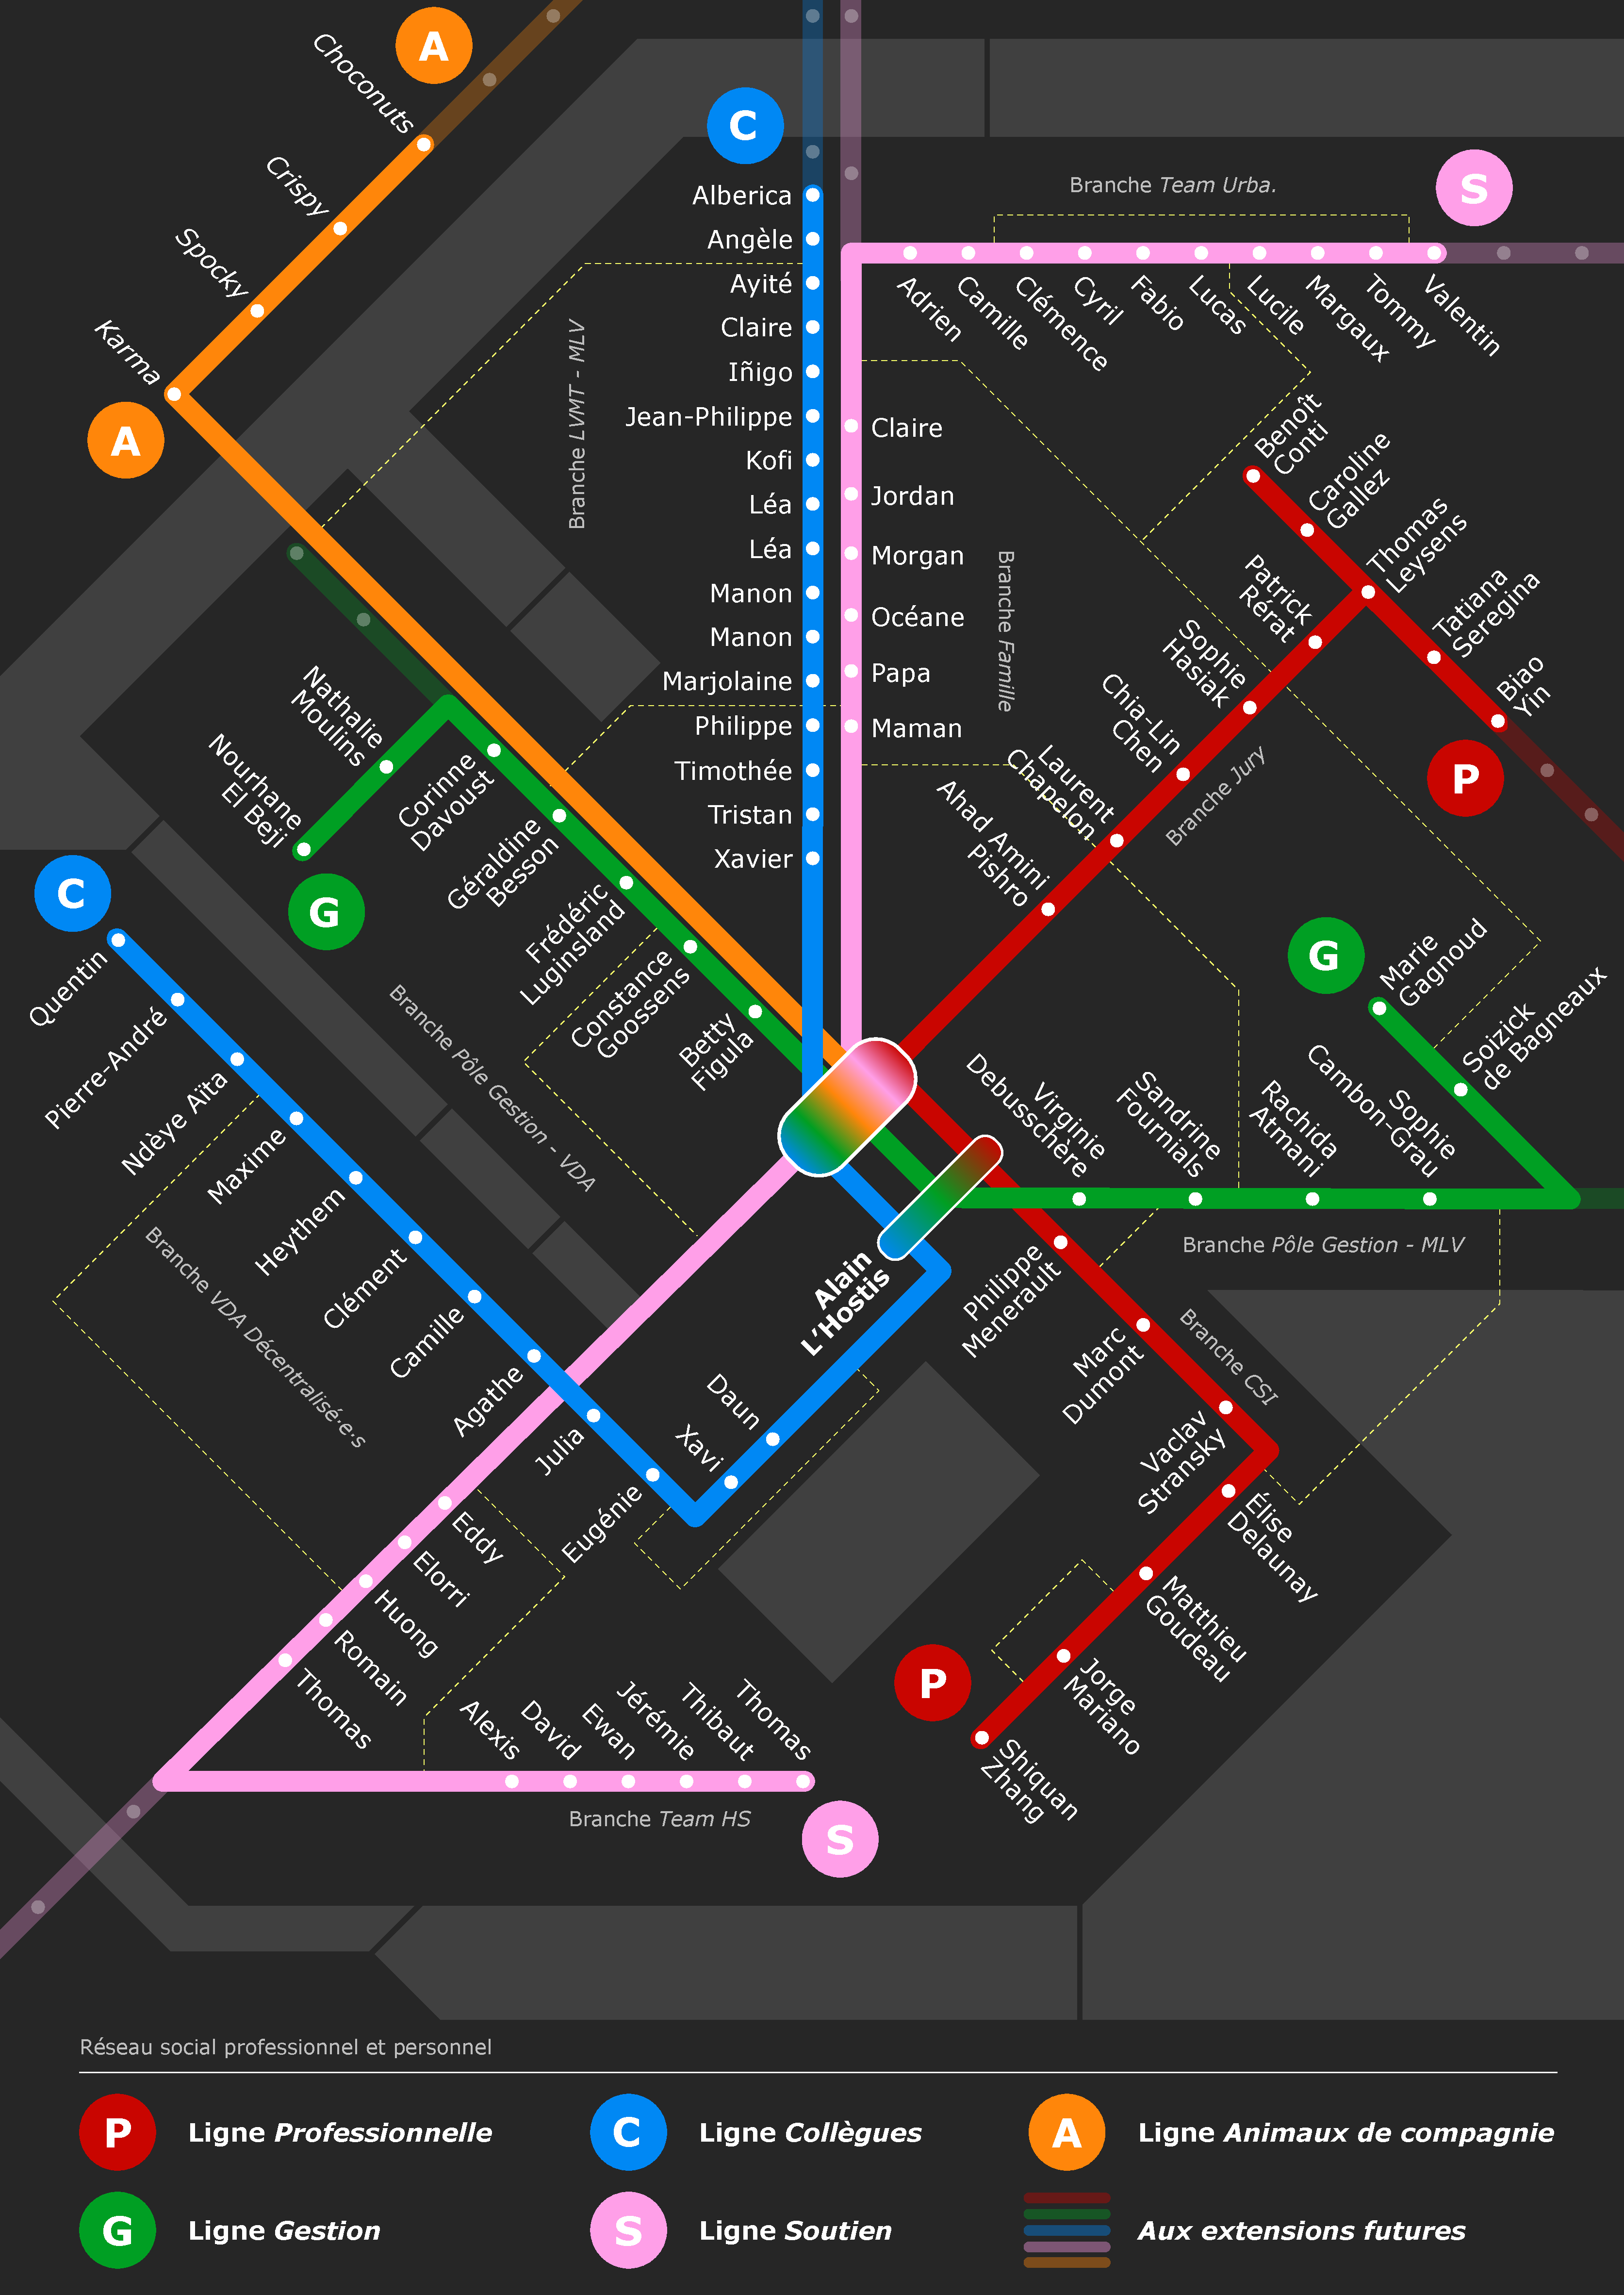
\includegraphics[width=1\columnwidth]{src/Figures/Preambule/FR_Remerciements.pdf}}
        \vspace{5pt}
        \begin{flushright}\scriptsize{
        Auteur~: \textcolor{blue}{Dylan Moinse (2024)}
        }\end{flushright}
    \end{carte}